\documentclass[letterpaper, 10 pt, conference]{ieeeconf} % letterpaper/a4paper 
% ieeeconf IEEEtran
\IEEEoverridecommandlockouts   % Needed if you want to use the \thanks command
\overrideIEEEmargins

\usepackage{amsmath} 
\usepackage{graphicx}
\usepackage[ruled,vlined]{algorithm2e}
\usepackage{amsfonts} % for mathbf and mathbb
\usepackage{hyperref} % required because bib generates \url{}
\usepackage{verbatim} % For begin{comment} end{comment}
\usepackage{authblk} % useful for multiple authors with different affiliations
\usepackage{cite} % useful to show multiple citations in single square bracket

\DeclareMathOperator*{\argmin}{arg\,min}
\DeclareMathOperator*{\argmax}{arg\,max}
\newcommand{\vect}[1]{\mathbf{#1}}
\newcommand{\hvect}[1]{\bar{\vect{#1}}}
\newcommand{\uvect}[1]{\hat{\vect{#1}}}
\newcommand{\field}[1]{\mathbb{#1}}
\newcommand{\Real}[0]{\field{R}}


\title{\Large \bf
Modern MAP methods for accurate and faster occupancy grid mapping
}
\author[1]{Vikas Dhiman}
\author[2]{Abhijit Kundu}
\author[2]{Frank Dallaert}
\author[1]{Jason J. Corso}
\affil[1]{{\tt\small\{vikasdhi,jcorso\}@buffalo.edu}}
\affil[1]{ Department of Computer Science and Engineering, SUNY at Buffalo, NY, USA }
\affil[2]{{\tt\small\{abhijit.kundu,frank\}@gatech.edu}}
\affil[2]{College of Computing, Georgia Tech, GA, USA}

\begin{document}
\maketitle
\begin{abstract}
  %JCorso: if you want to cite papers in the abstract, then you can add the 
  %\cite{thrun2003learning,merali2013icra}  back into the abstract, but I think 
  %this is a rare and not advised practice (citing in the abstract).
  %
  %JCorso: XXX: is the ``more accurate maps more efficiently'' correct?
Using the inverse sensor model has been popular in occupancy grid mapping. 
However, it is widely known that applying the inverse sensor model to mapping 
requires certain assumptions that are not necessarily true. Even work that uses 
forward sensor models have relied on methods like expectation maximization or 
Gibbs sampling which have been succeeded by more effective methods of maximum a 
posteriori (MAP) inference over graphical models. In this paper, we propose the 
use of modern MAP inference methods along with the forward sensor model.  Our 
implementation and experimental results demonstrate that these modern inference 
methods deliver more accurate maps more efficiently than previously used 
methods.
\end{abstract}
\section{Introduction}
% % Outline
% * [X] Describe the problem. How it is important for robotics?
% * [X] What are different ways of solving problem?
% * [X] Do we focus on a particular way of solving?
% * [X] What is the common trend?
% * [X] What is wrong  with current approach?
% * [X] What are we proposing?
% * [X] Has someone done this before? If yes, how are we different.

Mobile robot problems like navigation, path planning, localization and collision 
avoidance require an estimate of the robot's spatial environment; this 
underlying problem is called robot mapping\cite{thrun2002robotic}.  Even in 
environments where maps are available, the environment may change over time 
necessitating a mapping ability on the mobile robot.  Robot mapping hence 
remains an active field of research 
\cite{meyer2012occupancy,nagla2012improved,merali2013icra} as it is an important 
problem in application areas like indoor autonomous navigation, grasping, 
reconstruction and augmented reality.

% This paragraph just provides some information that should be widely known; I'm 
% not sure it should be included.  At the least, it can be removed if space is 
% an issue.
Although robot mapping can be performed in a many ways---metric or topological; 
with range sensors, like sonar \cite{thrun2003learning}, laser scanners 
\cite{thrun2003learning} and RGBD \cite{newcombe2011kinectfusion}, or 
bearing-only sensors \cite{davison2007monoslam,kundu2011realtime}---metric 
mapping with range sensors is the most common.  Bearing-only sensors provide 
estimates up to a scale factor; topological maps still require local metric 
estimates for certain problems like navigation.  We hence focus on metric 
mapping with range sensors, specifically, laser scanners.

Occupancy grid mapping (OGM) is a popular and useful range-based mapping methods 
\cite{elfes1989using,moravec1988sensor}.  It affords a simple implementation and 
avoids a need to explicitly seek and match landmarks in the environment 
\cite{XXX}.  In contrast, it discretizes the environment into cells, squares 
(2D) or cubes (3D), and associates a random variable with each cell that 
represents the probability of the cell being occupied or free.  


OGM methods vary in how cell occupancy is estimated (see Sec.  
\ref{sec:related}), but most of the occupancy grid mapping algorithms make use 
of an inverse sensor model by assuming that the occupancy of each cell can be 
estimated independently of the other cells in the map 
\cite{elfes1989using,moravec1988sensor,newcombe2011kinectfusion}.  The main 
reason for using this independence assumption is computational efficiency.  
However, the assumption is inaccurate and can lead to overconfident estimates of 
occupancy in noisy observations \cite{thrun2003learning,merali2013icra}. 

To overcome this limitation, Thrun \cite{thrun2003learning} proposes a forward 
sensor model and uses expectation maximization to estimate occupancy.  Following 
in this line of work, more recently, Merali et al. \cite{merali2013icra} defines 
a Gibbs sampling algorithm based on a conditional estimate of cell occupancy 
given the rest of the map.   Although these methods have relaxed the assumptions 
of independence, they remain computationally expensive and hence limited in 
applicability.  For example, it is widely known that Gibbs sampling is 
computationally expensive and can get caught in local maxima \cite{LiBOOK2002}.

In contrast, in this paper, we explore the use of modern inference algorithms 
for more effective occupancy grid mapping with forward sensor models.
Our contribution in this paper is two fold. Firstly, we introduce the factor
graph approach of approaching occupancy grid mapping problem, which, to the
best of our knowledge, has not been applied to this problem.   This factor graph 
formalism makes it plausible to apply modern fast inference algorithms, such as 
loopy belief propagation \cite{kschischang2001factor} and dual decomposition 
\cite{sontag2011introduction}.  

% TODO: Someone should verify, if this is a mentionable contribution.
Secondly, we introduce a class of higher order potentials for our factor graph 
approach.  Factor graph inference is exponential in neighborhood size, which 
requires us to focus on a certain sub-class of potentials for tractability, such 
as the linear constraint-nodes \cite{potetz2007efficient} or pattern-based 
potentials \cite{komodakis2009beyond}.  We extend the pattern-based potentials, 
which explicitly computes the potential only for certain factors matching a 
given set of patterns and otherwise assigns a constant.  Whereas the 
pattern-based potentials in \cite{komodakis2009beyond} define each pattern with 
a fixed value for each node, we generalize these pattern-based potentials by 
allowing for \textit{free} nodes whose value does not impact the computed 
marginal.  

We implement these contributions for effective occupancy grid mapping with a 
forward sensor model and test our work on both simulated and real-data. Our 
experiments demonstrate the effectiveness of our novel OGM approach, especially, 
dual decomposition.  


\section{Related work} 
\label{sec:related}

% History?
Moravec and Elfes \cite{elfes1989using,moravec1988sensor,moravec1985high} proposed the

\section{Related work}
Moravec and Elfes \cite{elfes1989using,moravec1988sensor,moravec1985high} 
proposed the
seminal work in occupancy grids mapping. While the proposed algorithm worked
well in practice and was computationally efficient, in some cases it provided
overconfident occupancy estimates. Thrun \cite{thrun2003learning} argued that
forward sensor models are theoretically as well as experimentally superior to 
inverse sensor models. He proposed the use of Expectation maximization
algorithm for inference. More recently, Merali et al. \cite{merali2013icra}
proposed the use of Gibbs sampling algorithm for occupancy grid mapping.

One of the main contribution of this paper is the application of modern MAP
algorithms on occupancy grid mapping. We apply sum product belief propagation 
\cite{kschischang2001factor} and dual decomposition
\cite{sontag2011introduction} to the mapping problem. Belief propagation
introduced by \cite{pearl1986fusion} was introduced as an algorithm to compute
marginals over graphs without loops.  Surprisingly, it was found to work well
on graph with loops, even though it is not guaranteed to converge. Later it
was found that the convergent solution to Belief propagation corresponds to
the minima of so-called Bethe free energy \cite{yedidia2000generalized}, which
not only provided a theoretical justification for application of belief
propagation to graphs with loops, but also solves the convergence problem by 
the existence of an objective function which can be minimized directly.

% http://www.timeanddate.com/countdown/generic?iso=20130916T03&p0=422&msg=ICRA+deadline&csz=1
\cite{wiegerinck2003fractional} Fractional belief propagation
\cite{wainwright2005map} TRW belief propagation.
\cite{kolmogorov2006convergent} TRW-S
\cite{meltzer2009convergent} unifying
\cite{jojic2010accelerated} Accelerated dual decomposition

Dual decomposition 



%Method of MAP inference have been subject to intensive
%research in the field of computer vision and information theory \cite{kappes2013comparative}.

% Work that has been in done in "method" that i.e MAP
Minimization of cost (or energy) function over Factor graphs is a well studied
field and it has found numerous application in the field of information theory,
computer vision and machine learning. A lot of work has been done in the field.

% Work on higher order potentials
\cite{leonardis2006efficient}  propose decreasing the labels set of variable
nodes to restrict the size of sample space of high order neighborhood. 

\section{Problem definition}
\newcommand{\map}{\vect{x}}
\newcommand{\measurements}{\vect{z}}
\newcommand{\poses}{\vect{\rho}}
A robot equipped with a laser scanner and accurate odometry moves in a static
environment, problem is to figure out an optimal occupancy grid map. For the
purpose of ground robots often 2D maps are enough for path planning and
exploration.
% define problem in probability terms
The area to be mapped is divided into $N$ discrete cells. Let $x_i$ denote the
state of cell $i$, which can take values from label set $L_i = \{0, 1\}$, where
$0$ (resp. $1$) denotes that cell is free (resp. occupied). We define, the map
$\map$ as a set that defines state for all $N$ cells, $\map = [x_i]^\top_{1
\le i \le N}$. Hence map $\map$ takes values from sample space $\Omega =
\prod_{1 \le i \le N}L_i$.

Let $z_f$ denote the $f$\textsuperscript{th} laser range measurement when captured from pose $\rho_f$. 
%We assume that the probability of observation $p(z_f| \rho_f, \map)$ (forward sensor model) be given.
The problem is to find the probability of all cells of the map being occupied
given all $t$ observations, $z = [z_f]^\top_{1 \le f \le t}$ and
$\rho = [\rho_f]^\top_{1 \le f \le t}$.
\begin{align}
  p(x_i = 1 | \measurements, \poses) &= \sum_{\map \in \Omega : x_i = 1} p(\map | \measurements , \poses) & \forall 1 \le i \le N 
  \label{eq:fullsolution}
\end{align}
In another formulation of problem, we can focus on the best overall occupancy of the map that maximizes the posterior probability:
\begin{align}
  \vect{x}^* &= \argmax_{\map \in \Omega } p(\map | z, \rho)
  \label{eq:mapproblem}
\end{align}
% Clearly, \eqref{eq:mapproblem} is a simpler problem than
% \eqref{eq:fullsolution}. If problem is \eqref{eq:fullsolution} is solved than
% problem \eqref{eq:mapproblem} is solved by just taking the label that maximizes
% the marginal probability.
Both the problems \eqref{eq:fullsolution} and \eqref{eq:mapproblem} are related
problems but yield different results. While \eqref{eq:fullsolution} is
useful to keep track of uncertainty in an incremental fashion,
\eqref{eq:mapproblem} provides more meaningful result by providing a joint
occupancy configuration that maximizes posterior probability.

It is easy to see that any naive solution to any of the two problems would have complexity that is exponential in the number of cells. We can only hope to find an approximate solution of this problem.

\section{Mapping by inverse sensor model}
% assume independence
%\eqref{eq:fullsolution} is usually simplified in robotic mapping algorithms by introducing two assumptions:
Commonly used occupancy grid mapping algorithms make simplifying assumption
that each grid cell is independent of all other map cells. 
%As a result instead of the static world assumption (\eqref{eq:staticWorldAssumption}), we use 
\begin{align}
  %p(z_t|x_i, \sigma_{1:t-1}, \rho_t) = p(z_t|x_i, \rho_t)
  p(x_i|\measurements, \rho) &= \frac{p(z_t, \rho_t|x_i, \sigma_{1:t-1})p(x_i|\sigma_{1:t-1})}
                         {p(z_t, \rho_t|\sigma_{1:t-1})}
\end{align}
% Thrun03ar : A common assumption in mapping is the static world assumption, which states that past sensor readings are conditionally independent given knowledge of the map \map, for any point in time t:
The current laser measurement $z_t$ are commonly assumed (static world assumption) \cite{thrun2003learning} to be independent of previous observations $\sigma_{1:t-1}$ given the map $x_i$ :
\begin{align}
  p(z_t, \rho_t|x_i, \sigma_{1:t-1}) &= p(z_t, \rho_t|x_i)
 \label{eq:staticWorldAssumption}
\end{align}
Using static world assumption (\eqref{eq:staticWorldAssumption}), we get:
\begin{align}
 p(x_i|\measurements, \rho) &= p(z_t, \rho_t|x_i)\frac{p(x_i|\sigma_{1:t-1})}
                                           {p(z_t, \rho_t|\sigma_{1:t-1})}\\
                 &= \frac{p(x_i|z_t, \rho_t)p(z_t,\rho_t)} {p(x_i)}\frac{p(x_i|\sigma_{1:t-1})}{p(z_t, \rho_t|\sigma_{1:t-1})}\\
                 &= \frac{1}{Z'}\frac{p(x_i|z_t, \rho_t)p(x_i|\sigma_{1:t-1})}{p(x_i)}\\
                 &= \frac{1}{Z'}\prod_{1\le f \le t} \frac{p(x_i|z_f, \rho_f)}{p(x_i)}
\end{align}
where $Z'$ is a normalizing factor that is independent of $x_i$.


\section{Mapping by forward sensor model}

   Here we present minimum assumption simplification of
   \eqref{eq:fullsolution} as done in \cite{thrun2003learning,merali2013icra}. 
   For conciseness, we use 
   %$\sigma_t = \{z_t, \rho_t\}$ to represent both range and pose of $t$\textsuperscript{th} laser measurement.
   %Similarly,
   $\sigma_{1:t-1} = \{z_{1:t-1}, \rho_{1:t-1}\}$ to represent all but
   $t$\textsuperscript{th} measurement. For a given map $\map$, the conditional
   probability of map being correct is
   \begin{align}
     p(\map | \measurements, \rho) &= p(\map | \sigma_{1:t-1}, z_t, \rho_t)\\
                    &= \frac{p(z_t|\map , \sigma_{1:t-1}, \rho_t)p(\map| \sigma_{1:t-1}, \rho_t)}
                            {p(z_t|\sigma_{1:t-1}, \rho_t)}
     \label{eq:recursivesol}
   \end{align}
   Static world assumption, $p(z_t|\map, \sigma_{1:t-1}, \rho_t) = p(z_t|\map, \rho_t)$, simplifies \eqref{eq:recursivesol} to :
   \begin{align}
     p(\map|\measurements, \rho) &= \frac{p(z_t|\map, \rho_t)p(\map| \sigma_{1:t-1}, \rho_t)}
                          {p(z_t|\sigma_{1:t-1}, \rho_t)}\\
                  &= \frac{p(z_t|\map, \rho_t)p(\rho_t|\map, \sigma_{1:t-1})p(\map| \sigma_{1:t-1})}
                          {p(z_t|\sigma_{1:t-1}, \rho_t)p(\rho_t|\sigma_{1:t-1})}
   \end{align}

   Another common assumption is that the pose of robot $\rho_t$ being independent of map $\map$:
   \begin{align}
     p(\rho_t|\map, \sigma_{1:t-1}) = p(\rho_t|\sigma_{1:t-1})
   \end{align}
   Using independent pose assumption, we get a recursive formula for \eqref{eq:recursivesol}
   \begin{align}
     p(\map | \measurements, \rho) &= \frac{1}{Z} p(z_t|\map , \rho_t)p(\map| \measurements_{1:t-1}, \rho_{1:t-1})\\
                       &= \frac{1}{Z} \prod_{1 \le f \le t} p(z_f|\map, \rho_f)
     \label{eq:map}
   \end{align}
   where $Z$ is a normalizing constant independent of $\map$. The term $p(z_f|\vect{x}, p_f)$ is the \emph{forward sensor model}. Thrun et al. \cite{thrun2003learning} approach this problem by expectation maximization, while Merali et al. \cite{merali2013icra} use Gibbs sampling to find approximate solution. In this paper, we explore modern explore modern methods of finding maximum a posteriori estimate of this problem.

   Modern MAP methods approach the problem \eqref{eq:map}, by making use of the fact that a laser measurement depends only on a small portion of the entire map:
   \begin{align}
     p(z_f |\vect{x}, \rho_f) = p(z_f|\vect{x}_f, \rho_f)
   \end{align}
   where $\vect{x}_f \subseteq \vect{x}$ is the small portion of the map on which the laser measurement $f$ depends. Rewriting, \eqref{eq:map} in new notation:
   \begin{align}
     p(\map | \measurements, \rho) &= \frac{1}{Z} \prod_{1 \le f \le t} p(z_f|\map_f, \rho_f)
     \label{eq:modernmap}
   \end{align}
   %However, the full solution is computationally intractable as its complexity is exponential in the number of cells.
%\end{comment}


\section{Representation as factor graph and Notation}
\label{sec:notation}
The problem of Occupancy grid mapping can be expressed as energy minimization
over a factor graph. Let all cells in the map be the variable nodes $V$ and all
the laser measurements be factor nodes $F$. 
There exists an undirected edge $(i, f)$, if and only if the laser
range measurement $p(z_f|\vect{x}, \rho_f)$ depends on the cell occupancy 
$x_i$. In this paper, we assume that laser range measurement depends on only
those cells that the laser passes through for given pose $\rho_f$. Though more
complicated models can lead to better accuracy, we show that with such a simple
model we are able to achieve better accuracy than methods tried so far.
Let $E$ be set of all such edges:
% Mathematically,
\begin{align}
  E = \{(i, f) : i \in V, f \in F, \text{laser $f$ passes through cell $i$}\}
\end{align}
This defines our factor graph representation of occupancy grid mapping $G = (V, F, E)$.

%Let $n(.)$ denote neighborhood in factor graph $G = \{V, F, E\}$.
%
%% unncessary
% i.e
% \begin{align}
%   n(k) &= \begin{cases}
%   \{f \in F: (i, f) \in E\} & \text{ if $k \in V$}\\
%   \{i \in V: (i, f) \in E\} & \text{ if $k \in F$}
%   \end{cases}
% \end{align}
%
% As before each cell $i \in V$ takes values
% from a discrete set of labels $L_i = \{0, 1\}$, where $0$ (respectively $1$) means that
% the cell is free (respectively occupied). Also denote the sample space of all the
% cells in the map as $\Omega = \prod_{i \in V} L_i$.

% Each laser measurement $f \in F$ corresponds to a function $\theta_f : \vect{x}_f \rightarrow \Real$ 
% that depends only on the labels of the neighboring cells, $\vect{x}_f = \{x_i\}_{i
% \in n(f)}$, and evaluates to an
% \emph{energy} value. Here $n(.)$ denotes the neighborhood in the factor graph $G$.
% The \emph{energy} can be thought as the negative log likelihood of the given
% state $\vect{x}_f$ being the correct state according to the laser measurement $f$.

% In this formulation, we seek to determine the label of all the map cells that
% maximizes the total likelihood across all measurements, which is equivalent to
% minimizing the total \emph{energy} over all factors.
We rewrite the problems \eqref{eq:fullsolution} and \eqref{eq:mapproblem} here
in generic notation, along with use of factorization obtained in
\eqref{eq:modernmap}, for generic explanation of algorithms.
\begin{align}
  P_i(x_i = l_i) &= \sum_{\map \in \Omega : x_i = l_i} P(\vect{x}) & \forall i \in V
  \label{eq:marginalgeneric}
  \\
     \vect{x}* &= \argmax_{\vect{x} \in \Omega} P(\vect{x})
  \label{eq:mapgeneric}
  \\
   P(\vect{x}) &= \frac{1}{Z}\prod_{f \in F} P_f(\vect{x}_f)
  \label{eq:factorizationgeneric}
\end{align}
where  $l_i \in L_i$ denote an element from the label set $L_i$ of node $i \in V$.
The equations \eqref{eq:fullsolution}, \eqref{eq:mapproblem} and
\eqref{eq:modernmap} correspond to \eqref{eq:marginalgeneric},
\eqref{eq:mapgeneric} and \eqref{eq:factorizationgeneric} respectively. Also
note the corresponding equivalence of notation, $P_i(x_i = l_i) = p(x_i = l_i|z, \rho)$, $P(\vect{x}) = p(\vect{x}|z, \rho)$ and $P_f(\vect{x}_f) = p(z_f|\vect{x}_f, \rho_f)$.

Often, for computational reasons, this problem is approached in negative log
likelihood or \emph{energy} domain. Let 
$\theta_f(\vect{x}_f) = - \log P_f(\vect{x}_f)$ 
denote the \emph{energy} for the laser measurement $f$. Note that here we
assume that $P_f(\map_f) > 0$, which is practically achievable by
choosing very low probability values instead of zero for highly improbable
cases. We will be using this non-zero probability assumption for the rest of the paper. 
In energy domain, the problem \eqref{eq:mapgeneric}, along with
\eqref{eq:factorizationgeneric}, can be rewritten as
\begin{align}
  \vect{x}* = \argmin_{\vect{x} \in \Omega} \sum_{f \in F} \theta_f(\vect{x}_f)
\end{align}
\begin{figure}
  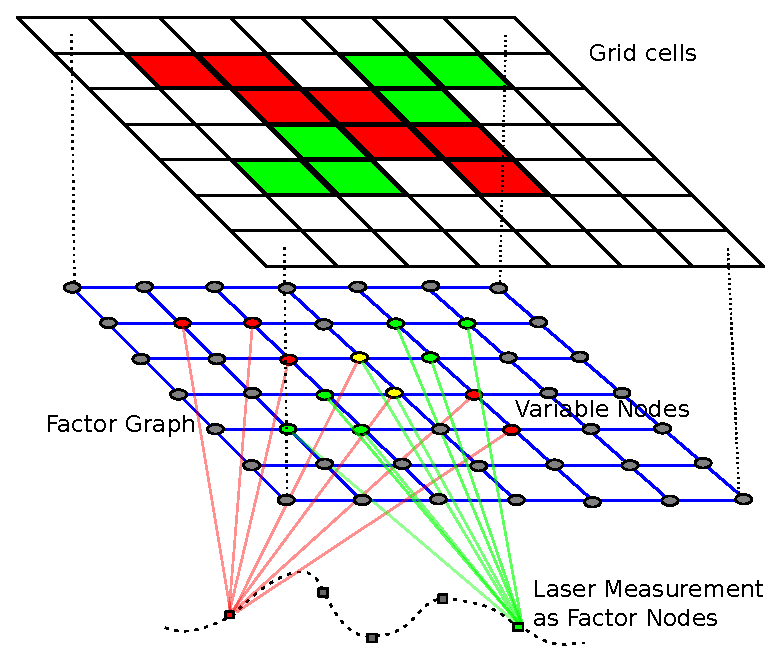
\includegraphics[width=\columnwidth]{../figures/factorgraph/factorgraph.pdf}
  \caption{Diagrammatic conversion of Occupancy Grid to a factor graph.}
  \label{fig:factor-graph}
\end{figure}

\section{Forward sensor models}
We explore here a few plausible sensor models
\subsection{Gaussian sensor model}
\newcommand{\actz}{\bar{z}_f(\vect{x}_f, \rho_f)}
In this sensor model, we assume that the laser measurements are affected by Gaussian noise. The forward sensor model is given by
\begin{align}
  p(z_f|\vect{x}_f, \rho_f) &=
  \frac{1}{\sqrt{2\pi}\sigma}\exp\left(-\frac{(\actz - z_f)^2}{2\sigma^2}\right)
  \label{eq:gaussiansensormodel}
\end{align}
where $\actz$ is the distance of first occupied cell in $\vect{x}_f$ starting from pose $\rho_f$. Also $\sigma$ is a measure of noise in laser measurement and it often depends on the distance measured. For our experiments we assume noise to linearly vary with distance as $\sigma = \sigma_0z_f$. 

In terms of negative log likelihood, the energy function becomes
\begin{align}
  \theta_f(\vect{x}_f) &= \frac{1}{2\sigma_0^2}\left(1 -
  \frac{\actz}{z_f}\right)^2 + \log(\sqrt{2\pi}\sigma_0z_f)
\end{align}
% In terms of discrete set of cells that the laser passes through the energy function becomes
% \begin{align}
%   \theta_f(\vect{x}_f) &= \frac{1}{\sigma_0^2}\left(1 - \frac{\kappa(\vect{x}_f) \Delta}{z_f}\right)^2 + \log(2\pi\sigma_0z_f)
% \end{align}
% where $\kappa(\vect{x}_f)$ denote the index of the first occupied cell in $\vect{x}_f$ and $\Delta$ is the cell size.

\subsection{Piecewise constant sensor model}
The expected pattern of occupancy from a laser observation is two have last cell as occupied and others as free. So the simplest energy function would be 
\begin{align}
  \theta_f(\vect{x}_f) &= \begin{cases}
              0 & \text{ if } \vect{x}_f = [0, 0 \dots 0, 1]^\top\\
           1000 & \text{ otherwise}
  \end{cases}
\end{align}
where $[0, 0 \dots 0, 1]$ means that all cells are $0$ except the last cell which is $1$. In this context, we consider $\vect{x}^f$ to be a vector of ordered cell labels through which laser measurement $f$ passes.

However, to resolve conflicts it is sometimes better to provide lower energy to all cells free case. Hence, we come with the following energy function.
\begin{align}
  \theta_f(\vect{x}_f) &= \begin{cases}
                     0 & \text{ if } \vect{x}_f = \vect{R}_1\\
                   900 & \text{ if } \vect{x}_f = \vect{R}_2\\
                  1000 & \text{ otherwise}
  \end{cases}
  \label{eq:piecewiseconstant}
\end{align}
where $\vect{R}_1 = [0, 0 \dots 0, 1]^\top$ and $\vect{R}_2 = [0, 0 \dots 0, 0]^\top$.

\subsection{Pattern-based functions}
\label{sec:patternfunctions}
However, we can efficiently compute \eqref{eq:factor2node} for certain class of
$P_f(.)$. Here, we take a consider a class of \emph{pattern-based} function
that are similar (yet different) to those discussed by Komodakis et al
\cite{komodakis2009beyond}. Pattern based functions are functions of the form:
\begin{align}
  P_f(\vect{x}_f) = \begin{cases}
    \psi_{1} & \text{ if $\vect{x}_f \sim \vect{R}_1$}\\
            .&.\\
    \psi_{m} & \text{ if $\vect{x}_f \sim \vect{R}_m$}\\
            .&.\\
    \psi_{\text{min}} & \text{ otherwise}
  \end{cases}
  \label{eq:patternfunction}
\end{align}
where $\vect{R}_m$ is one of the mutually exclusive $M$ patterns and operator
$\vect{x}_f \sim \vect{R}_m$ denotes that vector $\vect{x}_f$ matches pattern
$\vect{R}_m$.  
%Usually $M$ is either a constant or linear in the size of neighborhood $n(f)$.
%We further constrain the class of functions by requring each pattern
A pattern $\vect{R}_m$ is defined by a non empty set of \emph{fixed} nodes
$n^m_0(f) \subseteq n(f)$ from neighboring nodes to have fixed values $\vect{r}_m$, 
while the state of remaining \emph{free} nodes $n^m_*(f) = n(f) \setminus
n^m_0(f)$ can have any values and they do not affects $P_f(\vect{x}_f)$.
We assume that the number
of patterns $M$ is much smaller than the sample space of $\vect{x}_f$.

Here, we show that gaussian sensor
model \eqref{eq:gaussiansensormodel} can also be represented as pattern based function. 
We use the fact that the term $\bar{z}_f(\vect{x}_f, \rho_f)$, just depends on
first occupied cell. We define pattern $\vect{R}_m$ such that the first
occupied cell is $m$\textsuperscript{th} cell in $n(f)$:
\begin{align}
  \vect{x}_f \sim \vect{R}_m = \begin{cases}
    1 & \text{ if $x_{fk} = 0 \, \forall k < m$ and $x_{fm} = 1$}\\
    0 & \text{ otherwise}
  \end{cases}
\end{align}
where $x_{fk}$ is the $k$\textsuperscript{th} element in $\vect{x}_f$. With
this formulation, we will have $M = n(f)$ patterns to describe the gaussian
sensor model in the form \eqref{eq:patternfunction} with $\psi_m$ given by
\begin{align}
  \psi_m &= \frac{1}{\sqrt{2\pi}\sigma}\exp\left(-\frac{(\delta(m)- z_f)^2}{2\sigma^2}\right)
\end{align}
where $\delta(m)$ is the distance of $m$\textsuperscript{th} cell from robot
starting point $\rho_f$. Also note that in this formulation the only case for
\emph{otherwise} is the one when all cells are $0$ (or free).

It is clear that piecewise constant sensor model \eqref{eq:piecewiseconstant}
%Here we show that piecewise constant sensor model \eqref{eq:piecewiseconstant}
is an instance of pattern based functions.
%The first two cases of
%\eqref{eq:piecewiseconstant} are already in pattern-based format, but the
%otherwise case is not mutually exclusive with 

\section{Metropolis Hastings}
Markov Chain Monte Carlo (MCMC) methods allow us to sample from high dimensional probability distributions. The samples drawn using MCMC methods are not independent but correlated as a Markov chain. They work by moving in a random walk in the high dimensional space. Metropolis Hastings is one of the popular MCMC methods. The idea is to sample $\vect{x}$ from the probability distribution $p(\vect{x}|z, \rho)$ and after sufficient number of iterations, we should get sample that is close to the true map.

In general, for Metropolis hastings a \emph{transition probability} $Q(\vect{x}',
\vect{x}^r)$ is chosen, that depends on current sample $\vect{x}^r$ and guides
the random walk in the high-dimensional space. We randomly sample a point
$\vect{x}'$ from from $Q(.)$ and it is either accepted or rejected based on the
acceptance probability $a$:
\begin{align}
  a = \frac{P(\vect{x}')Q(\vect{x}^r, \vect{x}')}
  {P(\vect{x}^r)Q(\vect{x}', \vect{x}^r)}
\end{align}

If $a \ge 1$, then the new point $\vect{x}'$ is accepted otherwise it is accepted with probability $a$. Here acceptance means that the point in next iteration is taken as the sampled point otherwise the older point is retained:
\begin{align}
  \vect{x}^{r+1} = \begin{cases}
    \vect{x}' & \text{ if $\vect{x}'$ accepted}\\
    \vect{x}^r & \text{ otherwise}\\
  \end{cases}
\end{align}
Interested reader is referred to \cite{mackay1998introduction} for further details about the Metropolis Hastings algorithm.

For our problem, we need to sample map $\vect{x}$ from the probability
distribution $p(\vect{x}|z, \rho)$. Note that when the transition probability
is symmetric, for example Gaussian distribution, the acceptance probability is
simply the ratio of probabilities at the proposed point and the current point.
We uniformly sample from all the cells in the map and flip the state of the
sampled cell to get the proposal point $\vect{x}'$. Clearly, this transition probability is symmetric.
% TODO: how to write this distribution in
\begin{align}
  Q(\vect{x}', \vect{x}^r) = \begin{cases}
    \frac{1}{N} & \text{if $\|\vect{x}' - \vect{x}^r\|_1 = 1$}\\
      0 & \text{ otherwise}
  \end{cases}
  \label{eq:transitionprob}
\end{align}
where $N$ is the number of cells in the map and $\|.\|_1$ is the L1-norm. The
first case in \eqref{eq:transitionprob} enforces that only one cell (or dimension)
in the map
can change its state at a time. We will see this choice is one of the reasons of
poor performance of Metropolis Hastings. Also note that the ratio of probability distributions can be simplified by using \eqref{eq:factorizationgeneric}
\begin{align}
  a &= \frac{P(\vect{x}')}{P(\vect{x}^r)}\\
    &= \frac{\prod_{f \in F} P_f(\vect{x}'_f)}{\prod_{f \in F} P_f(\vect{x}^r_f)}\\
    &= \frac{\prod_{f \in n(i)} P_f(\vect{x}'_f)}{\prod_{f \in n(i)} P_f(\vect{x}^r_f)}
  \label{eq:acceptanceprob}
\end{align}
where $i$ is the cell whose state is different in $\vect{x}'$ and $\vect{x}^r$,
and $n(.)$ denotes the neighborhood of a vertex in graph $G$.

The above simplification uses the fact that only those terms  that depend on
state of $i$\textsuperscript{th} cell need to be computed. By definition
of graph $G$ only the neighboring factors $f \in n(i)$ depend on state of cell $i$.

% Now, we know that $\vect{x}'$ and $\vect{x}^r$ differ only by one cell or dimension, say $i$. Using this fact we can assert that only those subsets $\vect{x}_f$ of map can be different that contain
% 
\begin{algorithm}
  \KwData{
  Factor Graph $G = (V, F, E)$\;
  %Label set $\{\Sx\}_{i \in V}$\;
  %Step size $\alpha > 0$\;
  Maximum number of iterations $N$\;
  }
  \KwResult{$\vect{x}^r$}
  Initialize the map $\vect{x}^0$ randomly.\;
  $r = 0$\;
  \While {$r < N$} {
    Randomly choose a cell $i : i \in V$\;
    Flip its state $x'_i = \neg x^r_i$ in $\vect{x}^r$ to get $\vect{x}'$\;
    Compute acceptance probability $a$ by \eqref{eq:acceptanceprob}\;
    Sample random number $q : 0 \le q \le 1$\;
    \If {$a \ge 1$ or $a \ge q$} {
      Accept proposed point, $\vect{x}^{r + 1} = \vect{x}'$\;
    } \Else {
      Reject proposed point, $\vect{x}^{r + 1} = \vect{x}^r$\;
    }
    $r \leftarrow r + 1$\;
  }
  \caption{Metropolis Hastings}
\end{algorithm}

\subsection{Heat map}
As we uniformly sampled cells from the map, we noticed that not all
cells are equally important in mapping. There are three kinds of region any
occupancy map, occupied, free and unexplored. Sampling and analyzing a cell in
unexplored region is not much helpful as we do not have any evidence for the
region. On the other hand, the central regions of free areas are not very
interesting as all factors usually agree on their state. The uncertainty lies
usually lies along the boundaries of free and occupied regions. This is the
region we want to focus on.

We employ a \emph{heat map} to bias our sampling along the boundaries of free and occupied regions. We maintain a vector of cells $\vect{x}_h$ that form the ``interesting'' region of the map. In our experiments, we take the last cell spanned by each laser measurement as an ``interesting'' cell and add it to the \emph{heat map}, $\vect{x}_h$. We use a sampling bias of $1:4$ for cells outside heat map to cells within heat map.

We observe that Metropolis Hastings algorithm converges faster by using \emph{heat map}.

\section{Sum product}
\newcommand{\msg}[4]{\mu^{#4}_{#1\rightarrow#2}(#3)}
% TODO: Use introduction section of \cite{potetz2007efficient} to introduct belief propagation specifically 
Sum product algorithm over factor graphs \cite{kschischang2001factor} is a
powerful yet simple algorithm to compute marginals  of
expression (of the form \eqref{eq:fullsolution}) that can be decomposed into
factors of the form \eqref{eq:modernmap}. The algorithm provides exact
marginals in the case when the graphs have no loops. For general case the
algorithm has been shown %TODO: cite?  
to converge in most of the practical problems.
 
%The sum product algorithm is one of the easiest algorithm to implement. 
The sum product algorithm works by sending messages along the edges of factor
graph. The messages can be understood as a belief of the source node
considering all other neighbors except the destination. These messages are
defined on a directed edge, with a different message value for each state of
the variable node involved. 

Let $\msg{f}{i}{l_i}{r}$ represent message from
node $i \in V$ to node $f \in F$ for state $x_i = l_i$ at any iteration $r$ of the
algorithm. With a similar convention we take $\msg{i}{f}{l_i}{r}$ to denote
update in opposite direction. We use the following equations to update the messages depending whether the direction of edge is from variable node to factor node or vice versa:
\begin{align}
  \msg{f}{i}{l_i}{r+1} &= \sum_{\vect{x}_f \in \Omega_f: x_i = l_i}P_f(\vect{x}_f)\prod_{j \in n(f) \setminus i}\msg{j}{f}{x_j}{r}
  \label{eq:factor2node}
  \\
  \msg{i}{f}{l_i}{r+1} &= \prod_{h \in n(i) \setminus f}\msg{h}{i}{l_i}{r}
  \label{eq:node2factor}
\end{align}
where $\Omega_f = \prod_{i \in n(f)} L_i$ denotes the sample space of the neighborhood of factor $f$ in graph $G$.

When the factor graph is a tree, then the recommended message update sequence
is two pass sequence. The messages are updated starting from leaves towards the
root node in the first pass, and from root node leaves in the second pass,
where we have freedom to choose the root node. However, for graphs with loops
various update sequences have been suggested of which easiest to implement is
random update sequence i.e. a random edge is selected from the graph for each iteration.

\subsection{Efficient sum product}
We note that for Occupancy grid mapping the neighborhood of nodes in factor
graph $G$ can be large. For example a typical laser scan might have maximum
range of up to 50 m, which can cover up to 500 cells event at 10cm resolution.
In such a factor graph, even the sample space $\Omega_f$ of neighbors
$n(f)$ of factor $f$ can be very large; of the order of $2^{500}$  in above
example. This makes message update step in \eqref{eq:factor2node}
computationally expensive.

To efficiently compute \eqref{eq:factor2node} for pattern-based functions defined Section~\ref{sec:patternfunctions}, we need the messages to be normalized. The messages $\msg{i}{f}{l_i}{r}$ are often normalized over the label set $L_i$ to sum up to one:
\begin{align}
  \sum_{l_i \in L_i} \msg{i}{f}{l_i}{r} = 1
\end{align}

Using this property, we can efficiently compute \eqref{eq:factor2node}. We
compute the probability of each pattern being true using messages as beliefs
$\msg{i}{f}{x_i}{r}$
\begin{align}
  &p(\vect{x_f} \sim \vect{R}_m) = \sum_{\vect{x_f} \sim \vect{R}_m} \prod_{j \in n(f)}\msg{j}{f}{x_j}{r}\\
  %&= \prod_{j \in n^m_0(f)}\msg{j}{f}{R_{mj}}{r}\underbrace{\sum_{\vect{x}^*_f \in \Omega^*_f}\prod_{j \in n^m_*(f)}\msg{j}{f}{x_j}{r}}_{=1\text{, because $\vect{R}_m$ do not contraints $n^m_*(f)$}}\\
  &= \prod_{j \in n^m_0(f)}\msg{j}{f}{R_{mj}}{r}\left(\sum_{\vect{x_f} \sim \vect{R}_m}\prod_{j \in n^m_*(f)}\msg{j}{f}{x_j}{r}\right)
\end{align}
where $R_{mj}$ is the fixed value of $j$\textsuperscript{th} node in pattern
$\vect{R}_m$. The summation inside the bracket evaluates to one, because
$\vect{x}_f \sim \vect{R}_m$ do not constraints state of any node in $n^m_*(f)$
by definition. Hence, the probability of pattern is just the product of beliefs
of fixed terms:
\begin{align}
  p(\vect{x_f} \sim \vect{R}_m)&= \prod_{j \in n^m_0(f)}\msg{j}{f}{R_{mj}}{r}.
\end{align}

Unlike \eqref{eq:factor2node}, we do not leave out target node
$i$ from product terms, instead we temporarily replace the beliefs
$\msg{i}{f}{x_i}{r}$ with deterministic values to obtain the same effect
\begin{align}
  \msg{i}{f}{x_i}{r} = \begin{cases}
    1 & \text{if $x_i = l_i$}\\
    0 & \text{otherwise}
  \end{cases}
\end{align}
%Note that probabiltiy $p(\vect{x_f} \sim \vect{R}_m)$, depends only on the fixed nodes $n^m_0(f)$.
Now, we are in position to compute \eqref{eq:factor2node}
\begin{align}
  \msg{f}{i}{l_i}{r+1} &= \sum_{m \le M} \psi_m p(\vect{x_f} \sim \vect{R}_m)
  + \psi_{\text{min}} p_{\text{otherwise}}
  \label{eq:efficientbp}
\end{align}
where $p_{\text{otherwise}} = 1 - \sum_{m \le M}p(\vect{x_f} \sim \vect{R}_m)$.

The message update can be computed in $O(M|n(f)|)$ using \eqref{eq:efficientbp}, instead of $O(L_i^{n(f)-1})$ in the general case.

\section{Dual decomposition}
\renewcommand{\msg}[3]{\mu_{#1#2}(#3)}
\newcommand{\assign}{\leftarrow}
\newcommand{\Sx}{L_i}
Dual decomposition algorithm employs Lagrangian relaxation technique from
integer programming to minimize. Here we explain the implementation of the
algorithm without going into mathematical derivations. Interested user is
referred to
\cite{sontag2011introduction,jojic2010accelerated,komodakis2009beyond} for
proofs and more variations of the algorithm. 

Pseudo code for Dual decomposition is provided in
Alg~\ref{alg:dualdecompostion}. Apart from input factor graph $G = (V, F, E)$
and label set $\{\Sx\}_{i \in V}$ introduced in Sec~\ref{sec:notation}, Dual
decomposition depends on a step size $\alpha$.

The idea for Dual decomposition is to split the minimization problem into
\emph{slave} problems that can be efficiently minimized. In case of
disagreement for minimizing label among slave problems, the messages to slave
problems are updated until the slave problems agree with each other. We
maintain the minimizing label for variable node $i$, computed by slave problem
corresponding to $f$ as $x^f_i$. Also, we use $\msg{i}{f}{x_i}$ to denote
messages from node $i$ to slave problem corresponding to $f$ regarding state
$x_i$.

In each iteration of Dual Decomposition, we first minimize all the slave
problems getting labels for each pair of variable followed by message update in
case of disagreement. Optionally, we can only minimize only those factors that
have at least one disagreeing node in their neighborhood. However, the
performance gain obtained by such tweak is marginal.

\begin{algorithm}
  \dontprintsemicolon
  \KwData{\;
  Factor Graph $G = (V, F, E)$\;
  %Label set $\{\Sx\}_{i \in V}$\;
  Step size $\alpha > 0$\;
  Maximum number of iterations $N$\;
  }
  \KwResult{Labels $\{x^f_i\}_{(i, f) \in E} $,
  Messages $\{\msg{i}{f}{x_i}\}$}

  $\msg{i}{f}{x_i} \assign 0 \hfill \forall (i, f) \in E, x_i \in \Sx$\;
  $r \assign 1$\;
  \While{$r < N$} {
    %\tcp{For disagreeing factors}
    \For {$f \in F$} {% : \exists i, i' \in n(f) : x_i^f \ne x_{i'}^f$} {
      $\vect{x}^f \assign \argmin\limits_{\vect{x}^f} \left( \theta_f(\vect{x}^f) + \sum\limits_{i \in n(f)}\msg{i}{f}{x^f_i} \right)$\;
    }
    \tcp{For disagreeing nodes}
    \For {$i \in V : \exists f, f' \in n(i) : x_i^{f'} \ne x_i^f$} {
      \For{$f \in n(i)$}{
        $\msg{i}{f}{x^f_i} \assign \msg{i}{f}{x^f_i} + \frac{\alpha}{r}$\;
      }
    }
    $r \leftarrow r + 1$\;
  }
  \label{alg:dualdecompostion}
  \caption{Subgradient Dual Decomposition}
\end{algorithm}
We can compute the minimum energy assignment from dual decomposition messages.
\begin{align}
  x_i \assign \argmax\limits_{x_i \in \Sx} \sum\limits_{f \in n(i)} \msg{i}{f}{x_i}
\end{align}
However, the above computation is only valid if the node has at least a pair of disagreeing factors. In case of agreement, we simply take the agreed upon assignment or if the node is not connected to any factors, we take a random assignment.
%%%%%%%%%%%%%%%%%%%%%%%%%%%%%%%% Unncessary
% \begin{algorithm}
%   \dontprintsemicolon
%   \KwData{\;
%     The Variable Node $i \in V$\;
%     Factor Graph $G = (V, F, E)$\;
%     Label set $\Sx$\;
%     Labels $\{x^f_i\}_{f \in n(i)} $\;
%     Messages $\{\msg{i}{f}{x_i}\}$\;
%   }
%   \KwResult{Minimum energy label $x_i$}
%   \tcc{Check for disagreement}
%   \If{$\exists f, f' \in n(i) : x^{f'}_i \ne x^f_i$}{
%     $x_i \assign \argmax\limits_{x_i \in \Sx} \sum\limits_{f \in n(i)} \msg{i}{f}{x_i}$\;
%   } \Else {
%     \tcc{Take any agreed label}
%     $x_i \assign x^f_i : f \in n(i)$\;
%   }
%   \caption{Label from Dual decomposition messages }
%   \label{alg:compute-assignment}
% \end{algorithm}
%%%%%%%%%%%%%%%%%%%%%%%%%%%%%%%% Unncessary
\subsection{Efficient slave minimization}
Here we address the efficient slave minimization of pattern based functions (Sec.~\ref{sec:patternfunctions}). 
The problem is to minimize the energy function along with the received messages.
\begin{equation}
  \begin{split}
    \text{minimize }  S(\vect{x}_f) &=\theta_f(\vect{x}^f) + \sum_{i \in n(f)}\msg{i}{f}{x_i^f} \\
   \text{such that }  &\vect{x}^f \in \Omega_f
  \end{split}
\end{equation}
where $\theta_f(\vect{x}^f)$ is a pattern-based function of the form
\begin{align}
  \theta_f(\vect{x}^f) &= \begin{cases}
                \Psi_m & \text{ if $\vect{x}_f \sim \vect{R}_m$}\\
     \Psi_{\text{max}} & \text{ otherwise}
  \end{cases}
\end{align}

A general minimization algorithm will take time of the order that is
exponential in the number of cells a laser passes through as $\vect{x}^f$ can
have $|L_i|^{|n(f)|}$ possible values.
%However, minimizing pattern-based functions is relatively easy because 
We can compute minimum for each pattern case and then take the minimum among all the patterns. While computing minimum for single pattern we can make use of the fact that certain nodes are fixed while other free:
\begin{align}
  &\argmin_{\vect{x}_f \sim \vect{R}_m} S(\vect{x}_f) 
% &= \argmin_{\vect{x}_f \sim \vect{R}_m} \Psi_m + \msg{i}{f}{x_i^f}\\
  = \Psi_m + \argmin_{\vect{x}_f \sim \vect{R}_m} \sum_{i \in n(f)}\msg{i}{f}{x_i^f}\\
  &= \Psi_m + \sum_{i \in n^m_0(f)}\msg{i}{f}{R_{mi}} 
  + \argmin_{\vect{x}_f \sim \vect{R}_m} \sum_{i \in n^m_*(f)}\msg{i}{f}{x_i^f}
\end{align}

We have to still make sure that the \emph{otherwise} case is mutually
exclusive with all other patterns.  This can be done in two different ways,
depending on how big is the sample space for \emph{otherwise} case. If the
sample space for \emph{otherwise} case is small (like in the gaussian sensor
model), we simply go over all the entire sample space to find minimum value.
Otherwise, we depend on the sample space covered by patterns being small. In this case 
we keep finding best minimizations of $\sum_{i \in n(f)} \msg{i}{f}{x_i^f}$
untill we get a minimization that does not match any of the
patterns already considered. 
%If the number of patterns $M$ is small, we should
%be able to do this minimization efficiently.
% \begin{align}
%   \argmin_{\vect{x}_f \in \Omega_f} S(\vect{x}_f) &= \argmin_{m \le M} \argmin_{\vect{x}_f \sim \vect{R}_m} S(\vect{x}_f)
% \end{align}
% 
%\begin{align}
%    \min \theta_f(\vect{x}_f) = \min &\left( 0 + \sum_{\vect{x}_f = \vect{P}_1, i \in n(f)}\msg{i}{f}{x_i},\right.\\
%                            &900 + \sum_{\vect{x}_f = \vect{P}_2, i \in n(f)}\msg{i}{f}{x_i},\\
%                            &\left.1000 + \min_{\vect{x}_f \not\in \{\vect{P}_1, \vect{P}_2\}} \sum_{i \in n(f)}\msg{i}{f}{x_i} \right)
%\end{align}
For example, in case of piecewise constant sensor model, there are only two
patterns that need to be checked for exclusivity. The otherwise term can be
easily minimized by finding three best assignments that minimize 
$\sum_{i \in n(f)}\msg{i}{f}{x_i}$.

%choosing the minimizing state for each $i$ over all possible $\Omega(\vect{x}_f)$ by 
%simply choosing the minimizing $x_i \in L_i$ for each $i$. However, the
%minimizing labels can coincide with patterns $\vect{P}_1$ and $\vect{P}_2$. The
%solution is to find minimum three assignments of $\sum_{i \in
%n(f)}\msg{i}{f}{x_i}$ and pick the one that is not equal to $\vect{P}_1$ nor
%$\vect{P}_2$. 

%\subsection{Efficient slave minimization of piecewise constant factor}
%Minimizing slave problem can be done efficiently for specific kinds of functions, for example, piecewise constant functions.
%The problem is to minimize the energy function along with the received messages.
%\begin{align}
%  \min_{\vect{x}^f} \left( \theta(\vect{x}^f) + \sum_{i \in n(f)}\msg{i}{f}{x^f} \right)
%\end{align}
%A general minimization algorithm will take time of the order that is exponential in the number of cells a laser passes through as $\vect{x}^f$ can have $|L_i|^{|n(f)|}$ possible values. However, for our sensor model we can make use of the fact that the piecewise function needs to look for only two patterns. We should compute the total function value for these two patterns and the minimum value for the \emph{otherwise} case. 
%\begin{align}
%    \min \theta_f(\vect{x}_f) = \min &\left( 0 + \sum_{\vect{x}_f = \vect{P}_1, i \in n(f)}\msg{i}{f}{x_i},\right.\\
%                            &900 + \sum_{\vect{x}_f = \vect{P}_2, i \in n(f)}\msg{i}{f}{x_i},\\
%                            &\left.1000 + \min_{\vect{x}_f \not\in \{\vect{P}_1, \vect{P}_2\}} \sum_{i \in n(f)}\msg{i}{f}{x_i} \right)
%\end{align}
%The third term can be easily minimized by 
%%choosing the minimizing state for each $i$ over all possible $\Omega(\vect{x}_f)$ by 
%simply choosing the minimizing $x_i \in L_i$ for each $i$. However, the minimizing labels can coincide with patterns $\vect{P}_1$ and $\vect{P}_2$. The solution is to find minimum three assignments of $\sum_{i \in n(f)}\msg{i}{f}{x_i}$ and pick the one that is not equal to $\vect{P}_1$ nor $\vect{P}_2$. 
%
%%
%% Algorithm~\ref{alg:efficient-minimize} gives pseudo code for minimizing the last term.
%% \begin{algorithm}
%%   \SetKwFunction{ArgSortNElements}{ArgSortNElements}
%%   $e_i = \min\limits_{x_i \in L_i} \msg{i}{f}{x_i} \hfill, \forall i \in n(f)$\;
%%   $x^*_i = \argmin\limits_{x_i \in L_i} \msg{i}{f}{x_i} \hfill, \forall i \in n(f)$\;
%%   $\delta_{if}(x_i) = \msg{i}{f}{x_i} - e_i \hfill, \forall i \in n(f), x_i \in L_i, x_i \ne x^*_i$\;
%%   $I = \ArgSortNElements(\delta_{if}(x_i), \lceil{\log_{|L_i|}{3}}\rceil)$\;
%%   \caption{Efficient minimization of piecewise constant function}
%%   \label{alg:efficient-minimize}
%% \end{algorithm}

\subsection{Selection of step size}
Step size is critical choice as it affects the speed with which Dual decomposition converges. Fig~\ref{fig:dualdecomposition-stepsize} shows convergence with different step size.
\begin{figure}
  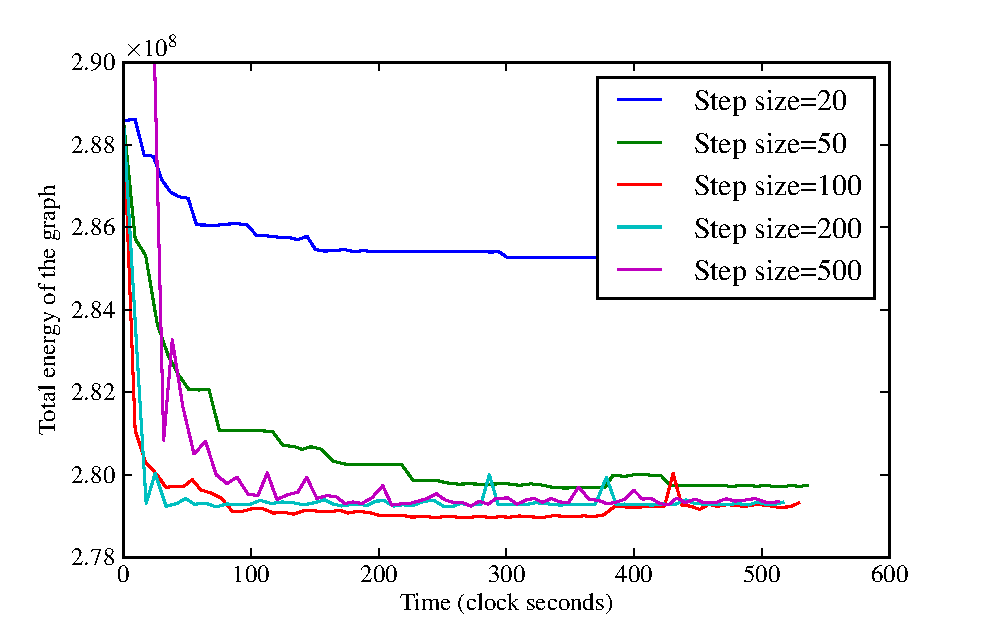
\includegraphics[width=\columnwidth]{../figures/dualdecomposition-stepsize-inc500.pdf}
  \caption{The rate of convergence in dual decomposition depends on step size}
  \label{fig:dualdecomposition-stepsize}
\end{figure}
% \section{Belief propagation with disagreement tracking}
% Intuitively, dual decomposition converges faster because it focuses on the disagreeing 

\section{Experiments} 
We run experiments on simulated as well real data.
The simulated data is generated using \emph{Player/Stage} \cite{gerkey2003player}
project. We use multiple map bitmaps bundled along with player/stage library.
The robot motion is generated using the wander driver. The robot is allowed to
wander in the map for 2 minutes aggregating approximately 270,000 laser measurements.
The qualitative results are shown in
Fig~\ref{fig:convergence-comparison-visuals} for several simulated dataset. To evaluate the
convergence rate of each algorithm, we plot total energy of the graph with
respect CPU ticks taken by the algorithm. The plot of energy convergence with respect to time for cave dataset is shown in Fig~\ref{fig:convergence-comparison}.

For real data, we have used the \emph{albert-b-laser} dataset provided by
Cyrill Stachniss from University of Freiburg. The dataset was captured by a
B21r robot with a SICK PLS moving through a lab at University of Freiburg.
This data set was obtained from the Robotics Data Set Repository
(Radish)~\cite{howard2003radish}. Thanks go to Cyrill Stachniss for providing
this data.

In all our experiments we do not use any occupancy prior. Although, Merali et
al \cite{merali2013icra} suggest using an occupancy prior of 0.3 for better
convergence. We use a step size of 50 for dual decomposition and piecewise constant 
sensor model.

\section{Conclusion}
We note that sampling algorithms are liable to getting stuck in a local minima
because we flip only one cell at a time. Even from the qualitative results for
sampling based algorithm, we see that the walls are thinner than corresponding
results in other algorithms which shows the inability of sampling based
algorithms to form lower energy thicker walls for piecewise constant sensor
model.

We note that dual decomposition is faster because it focuses on disagreeing
nodes. However, step size is crucial parameter that affects speed of
convergence. On the other hand sum product belief propagation do not depends
on any parameter factor, but has no preference for the disagreeing nodes.
This combination obviously hints towards an algorithm where we perform 
belief propagation over disagreeing nodes only. The state of art variations 
of these algorithms like Sequential Tree Re-Weighted (TRW-S) belief
propagation \cite{kolmogorov2006convergent}, accelerated dual Decomposition
\cite{jojic2010accelerated} are step in this direction.
However, even without using the state of art optimum algorithms since we get
better performance than sampling methods. This only serves to prove our
assertion that modern inference methods should be used occupancy grid mapping 
when computation time is not a limiting factor.

\begin{figure*}
  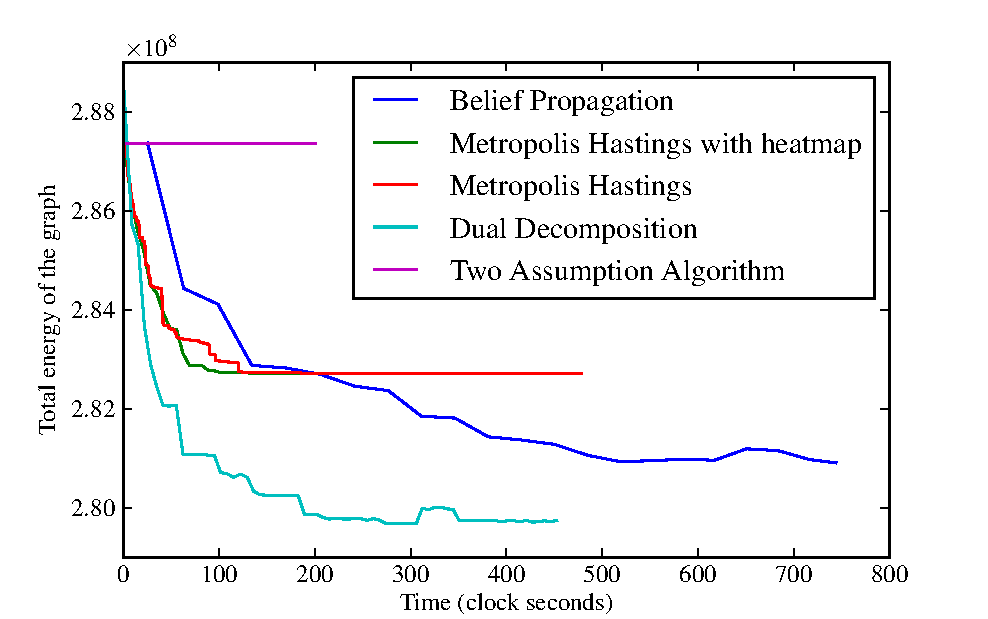
\includegraphics[width=0.24\textwidth]{../figures/relativeconvergence.pdf}%
  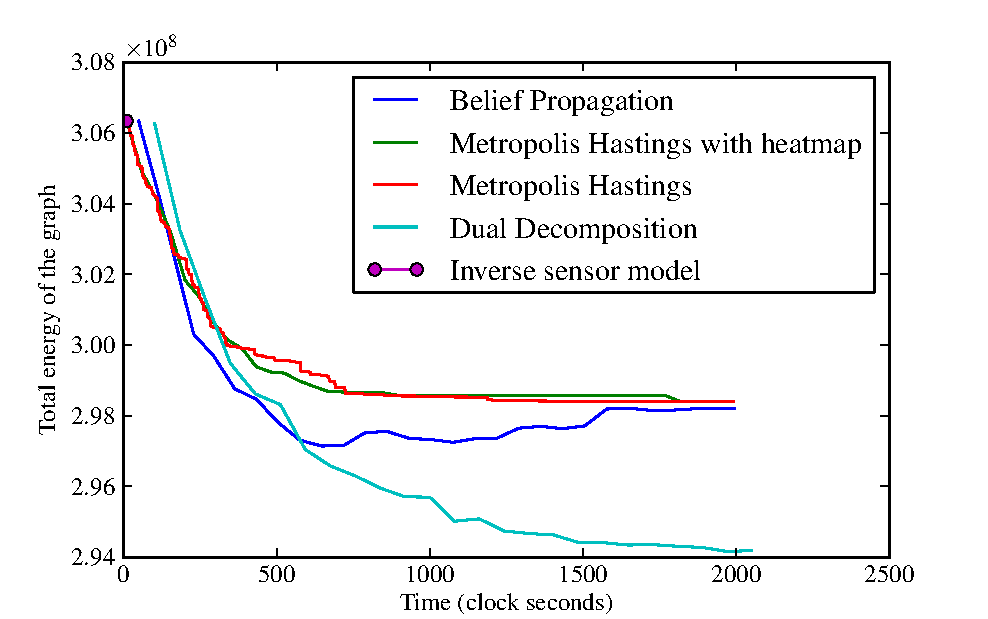
\includegraphics[width=0.24\textwidth]{../../Data/hospital_section_player/plot-time-energy.pdf}%
  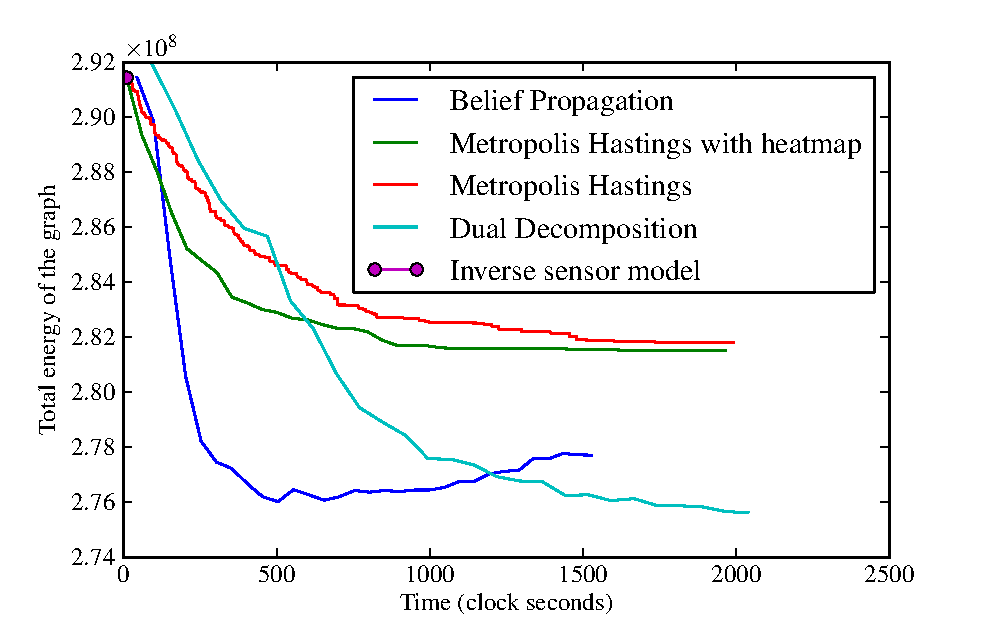
\includegraphics[width=0.24\textwidth]{../../Data/hospital_player/plot-time-energy.pdf}%
  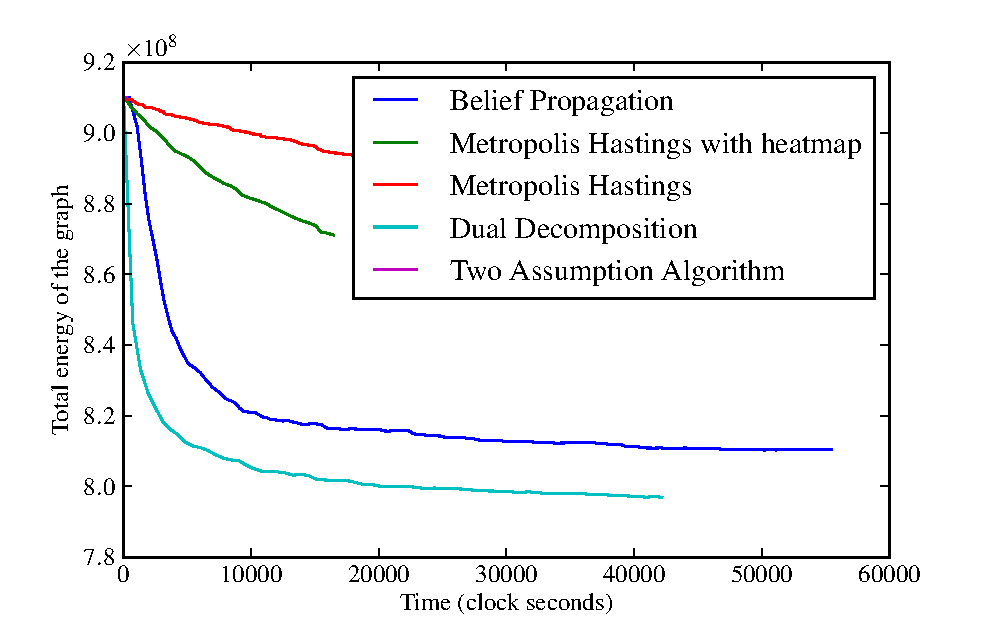
\includegraphics[width=0.24\textwidth]{../figures/convergence-albert-b.pdf}%
  \caption{Comparison of convergence of different algorithms on occupancy grid graph. While sampling methods like Metropolis hastings converge quickly they stay far from optimum energy. On the other hand modern minimization algorithms reach closer to an optimum value.}
  \label{fig:convergence-comparison}
\end{figure*}
\begin{figure*}
  %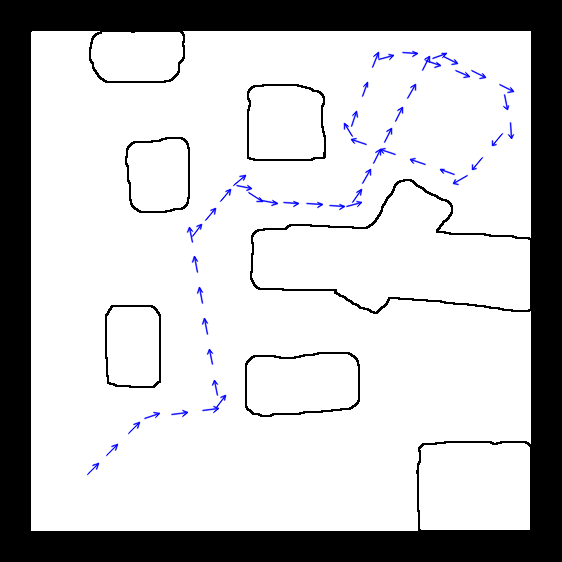
\includegraphics[width=0.2\textwidth]{../figures/cave_trajectory.png}%
  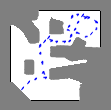
\includegraphics[width=0.16\textwidth]{../figures/cave_gt.png}%
  
\includegraphics[width=0.16\textwidth]{../figures/cave_TwoAssumptionAlgo.png}%
  
\includegraphics[width=0.16\textwidth]{../figures/cave_SICKSlowMetropolis.png}%
  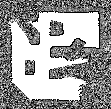
\includegraphics[width=0.16\textwidth]{../figures/cave_SICKDDMCMC.png}%
  
\includegraphics[width=0.16\textwidth]{../figures/cave_run_belief_propagation.png}%
  
\includegraphics[width=0.16\textwidth]{../figures/cave_dualdecomposition.png}\\
  
\includegraphics[width=0.16\textwidth]{../../Data/hospital_player/gt-final.png}%
  
\includegraphics[width=0.16\textwidth]{../../Data/hospital_player/TwoAssumptionAlgo.png}%
  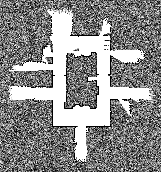
\includegraphics[width=0.16\textwidth]{../../Data/hospital_player/SICKSlowMetropolis.png}%
  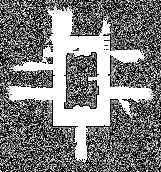
\includegraphics[width=0.16\textwidth]{../../Data/hospital_player/SICKDDMCMC.png}%
  
\includegraphics[width=0.16\textwidth]{../../Data/hospital_player/run_belief_propagation.png}%
  
\includegraphics[width=0.16\textwidth]{../../Data/hospital_player/dualdecomposition.png}\\
  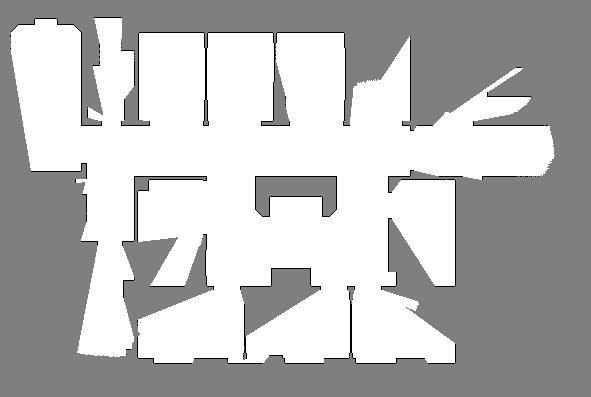
\includegraphics[width=0.16\textwidth]{../../Data/hospital_section_player/gt-final.png}%
  
\includegraphics[width=0.16\textwidth, trim=0 0 0 3px, clip]{../../Data/hospital_section_player/TwoAssumptionAlgo.png}%
  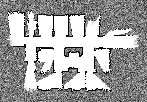
\includegraphics[width=0.16\textwidth, trim=0 0 0 3px, clip]{../../Data/hospital_section_player/SICKSlowMetropolis.png}%
  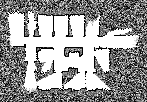
\includegraphics[width=0.16\textwidth, trim=0 0 0 3px, clip]{../../Data/hospital_section_player/SICKDDMCMC.png}%
  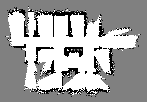
\includegraphics[width=0.16\textwidth, trim=0 0 0 3px, clip]{../../Data/hospital_section_player/run_belief_propagation.png}%
  
\includegraphics[width=0.16\textwidth, trim=0 0 0 3px, clip]{../../Data/hospital_section_player/dualdecomposition.png}%
  \caption{Qualitative results (from left to right) a) Ground truth with the trajectory of the robot b) Two assumption algorithm c) Metropolis Hastings without heat map d) Metropolis Hastings with heat map e) Belief Propagation  f) Dual decomposition. Each row represent a different simulated dataset.}
  \label{fig:convergence-comparison-visuals}
\end{figure*}

\begin{figure*}
  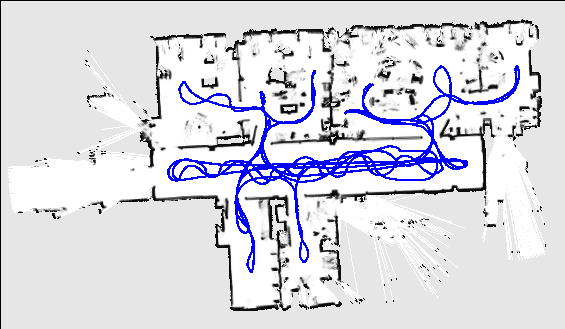
\includegraphics[width=0.33\textwidth]{../../Data/albertb.sm/path.png}%
  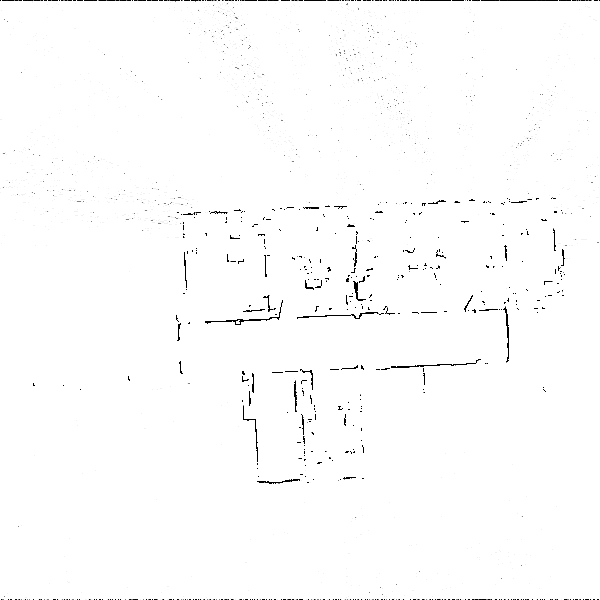
\includegraphics[width=0.33\textwidth, trim=65px 125px 20px 175px, clip]{../../Data/albertb.sm/TwoAssumptionAlgo.png}%
  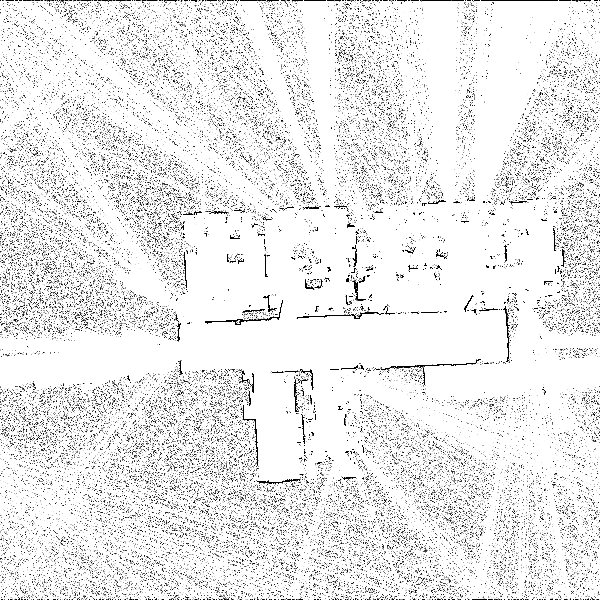
\includegraphics[width=0.33\textwidth, trim=65px 125px 20px 175px, clip]{../../Data/albertb.sm/SICKSlowMetropolis.png}\\
  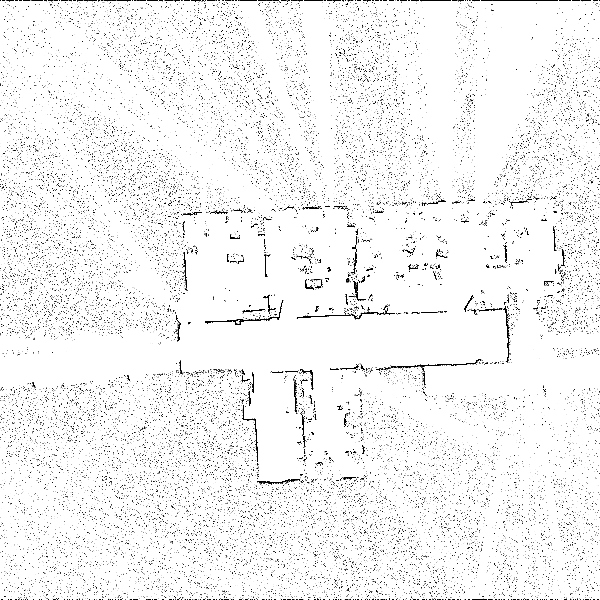
\includegraphics[width=0.33\textwidth, trim=65px 125px 20px 175px, clip]{../../Data/albertb.sm/SICKDDMCMC.png}%
  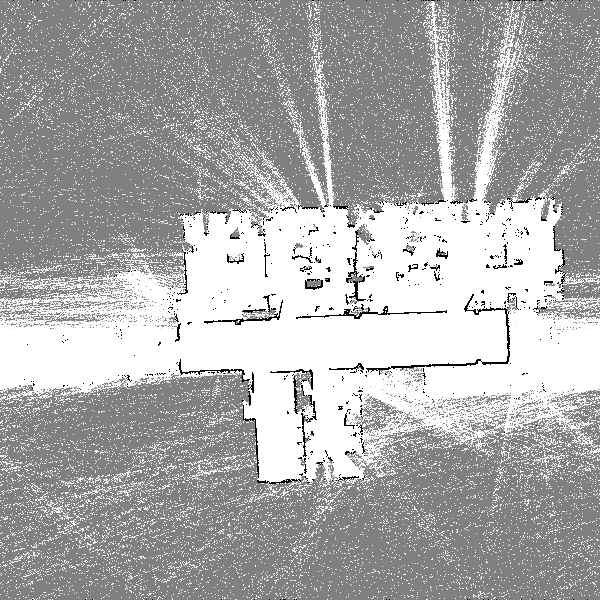
\includegraphics[width=0.33\textwidth, trim=65px 125px 20px 175px, clip]{../../Data/albertb.sm/run_belief_propagation.png}%
  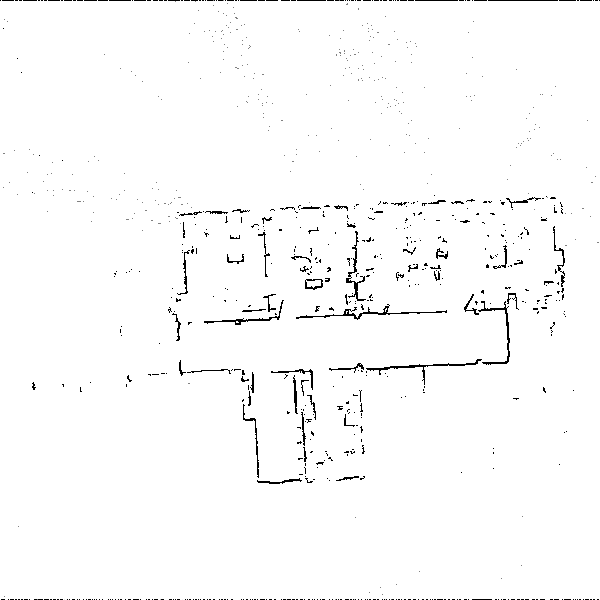
\includegraphics[width=0.33\textwidth, trim=65px 125px 20px 175px, clip]{../../Data/albertb.sm/dualdecomposition.png}%
  \caption{Qualitative results at the end of 200sec for each algorithm (from left to right) a) Ground truth with the trajectory of the robot b) Two assumption algorithm c) Metropolis Hastings without heat map d) Metropolis Hastings with heat map e) Belief Propagation  f) Dual decomposition}
  \label{fig:convergence-comparison-visuals-albertb}
\end{figure*}

\bibliographystyle{IEEEtran}
\bibliography{modern_map}
  
\end{document}

